\section{Décodeur 7 segment}
\subsection{Introduction}
\paragraph{}
Nous allons commencer par une prise en main de logisim en réalisant un décodeur 7 segments. Ce type d'afficheur est un grand classique en ce qui concerne l'affichage de caractères hexadécimaux.

\paragraph{}
Le principe de cet afficheur est très simple, En allumant plusieurs segments en même temps nous allons pouvoir représenter les caractères suivants :
0,1,2,3,4,5,6,7,8,9,A,B,C,D,E,F.

\begin{figure}[H]
        \makebox[\textwidth]{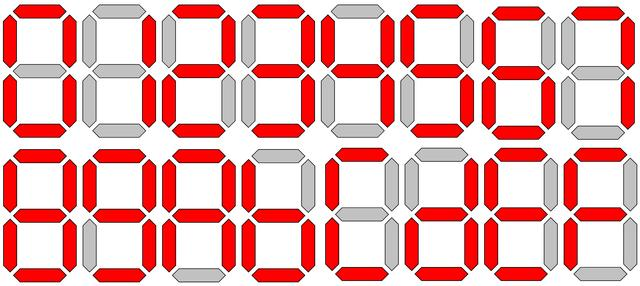
\includegraphics[width=15cm]{pictures/7seg.jpg}}
	\caption{Un affichage hexadécimal par 7 segments. Merci à @Skywodd - https://www.carnetdumaker.net/}
\end{figure}

\paragraph{}
L'objectif est ici est de recevoir une information sur 4 bits (comprise entre Ob0000 et 0b1111) et de la traduire sur 7 bits correspondant aux segments à allumer età ceux à éteindre.

\subsubsection{Table de correspondance}
Nous allons ici associer à chaque valeur à sa décomposition en segment d'après le schéma suivant :
\begin{figure}[H]
        \makebox[\textwidth]{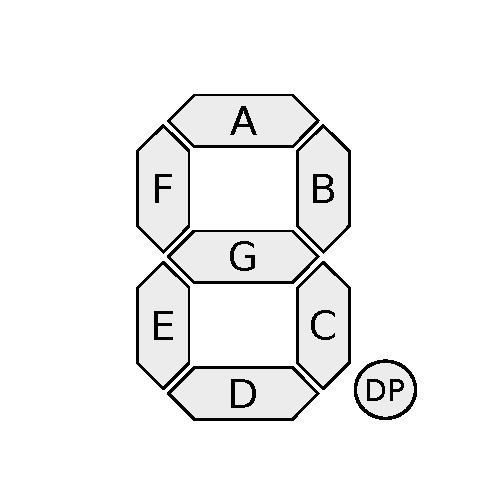
\includegraphics[height=3cm]{pictures/7segdetails.pdf}}
	\caption{Détail et Annotation d'un 7 segment par H2g2bob - logo}
\end{figure}
